  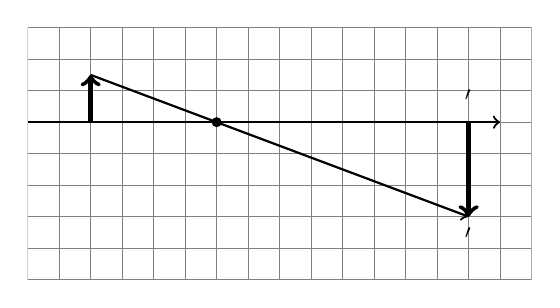
\begin{tikzpicture}[scale=0.8]
    \clip (-3,-2.5) rectangle (5,1.5) ; %Les dimensions de l'image
    \draw [help lines] (-3,-2.5) grid [step=0.5] (5,1.5) ; %% Le quadrillage
    \draw [->,thick] (-3,0) -- (4.5,0) ; %% L'axe optique


    \filldraw [black] (0,0) circle (2pt) node [above right] {$\ptO$} ;  %Le centre optique
    
      \draw [->,ultra thick] (-2,0) node [below] {$\ptA$} -- (-2,0.75) node [above] {$\ptB$} ;   %L'objet
      \draw [->,ultra thick] (4,0) node [above] {$\ptA'$} -- (4,-1.5) node [below] {$\ptB'$} ;  %L'image
      \draw [->,thick] (-2,0.75) -- (4,-1.5) ; %Le rayon lumineux reliant B et B'
      
  \end{tikzpicture}